\section{Routing}
This section contain general blockm scheme of SAYMA RTM board and I2C map with addresses. General Block Scheme -figure \ref{BlockScheme}
shows more important connections between components. I2C connections with addresses can be found in figure \ref{I2C}.
	\begin{figure}[htbp!]
		\centering
		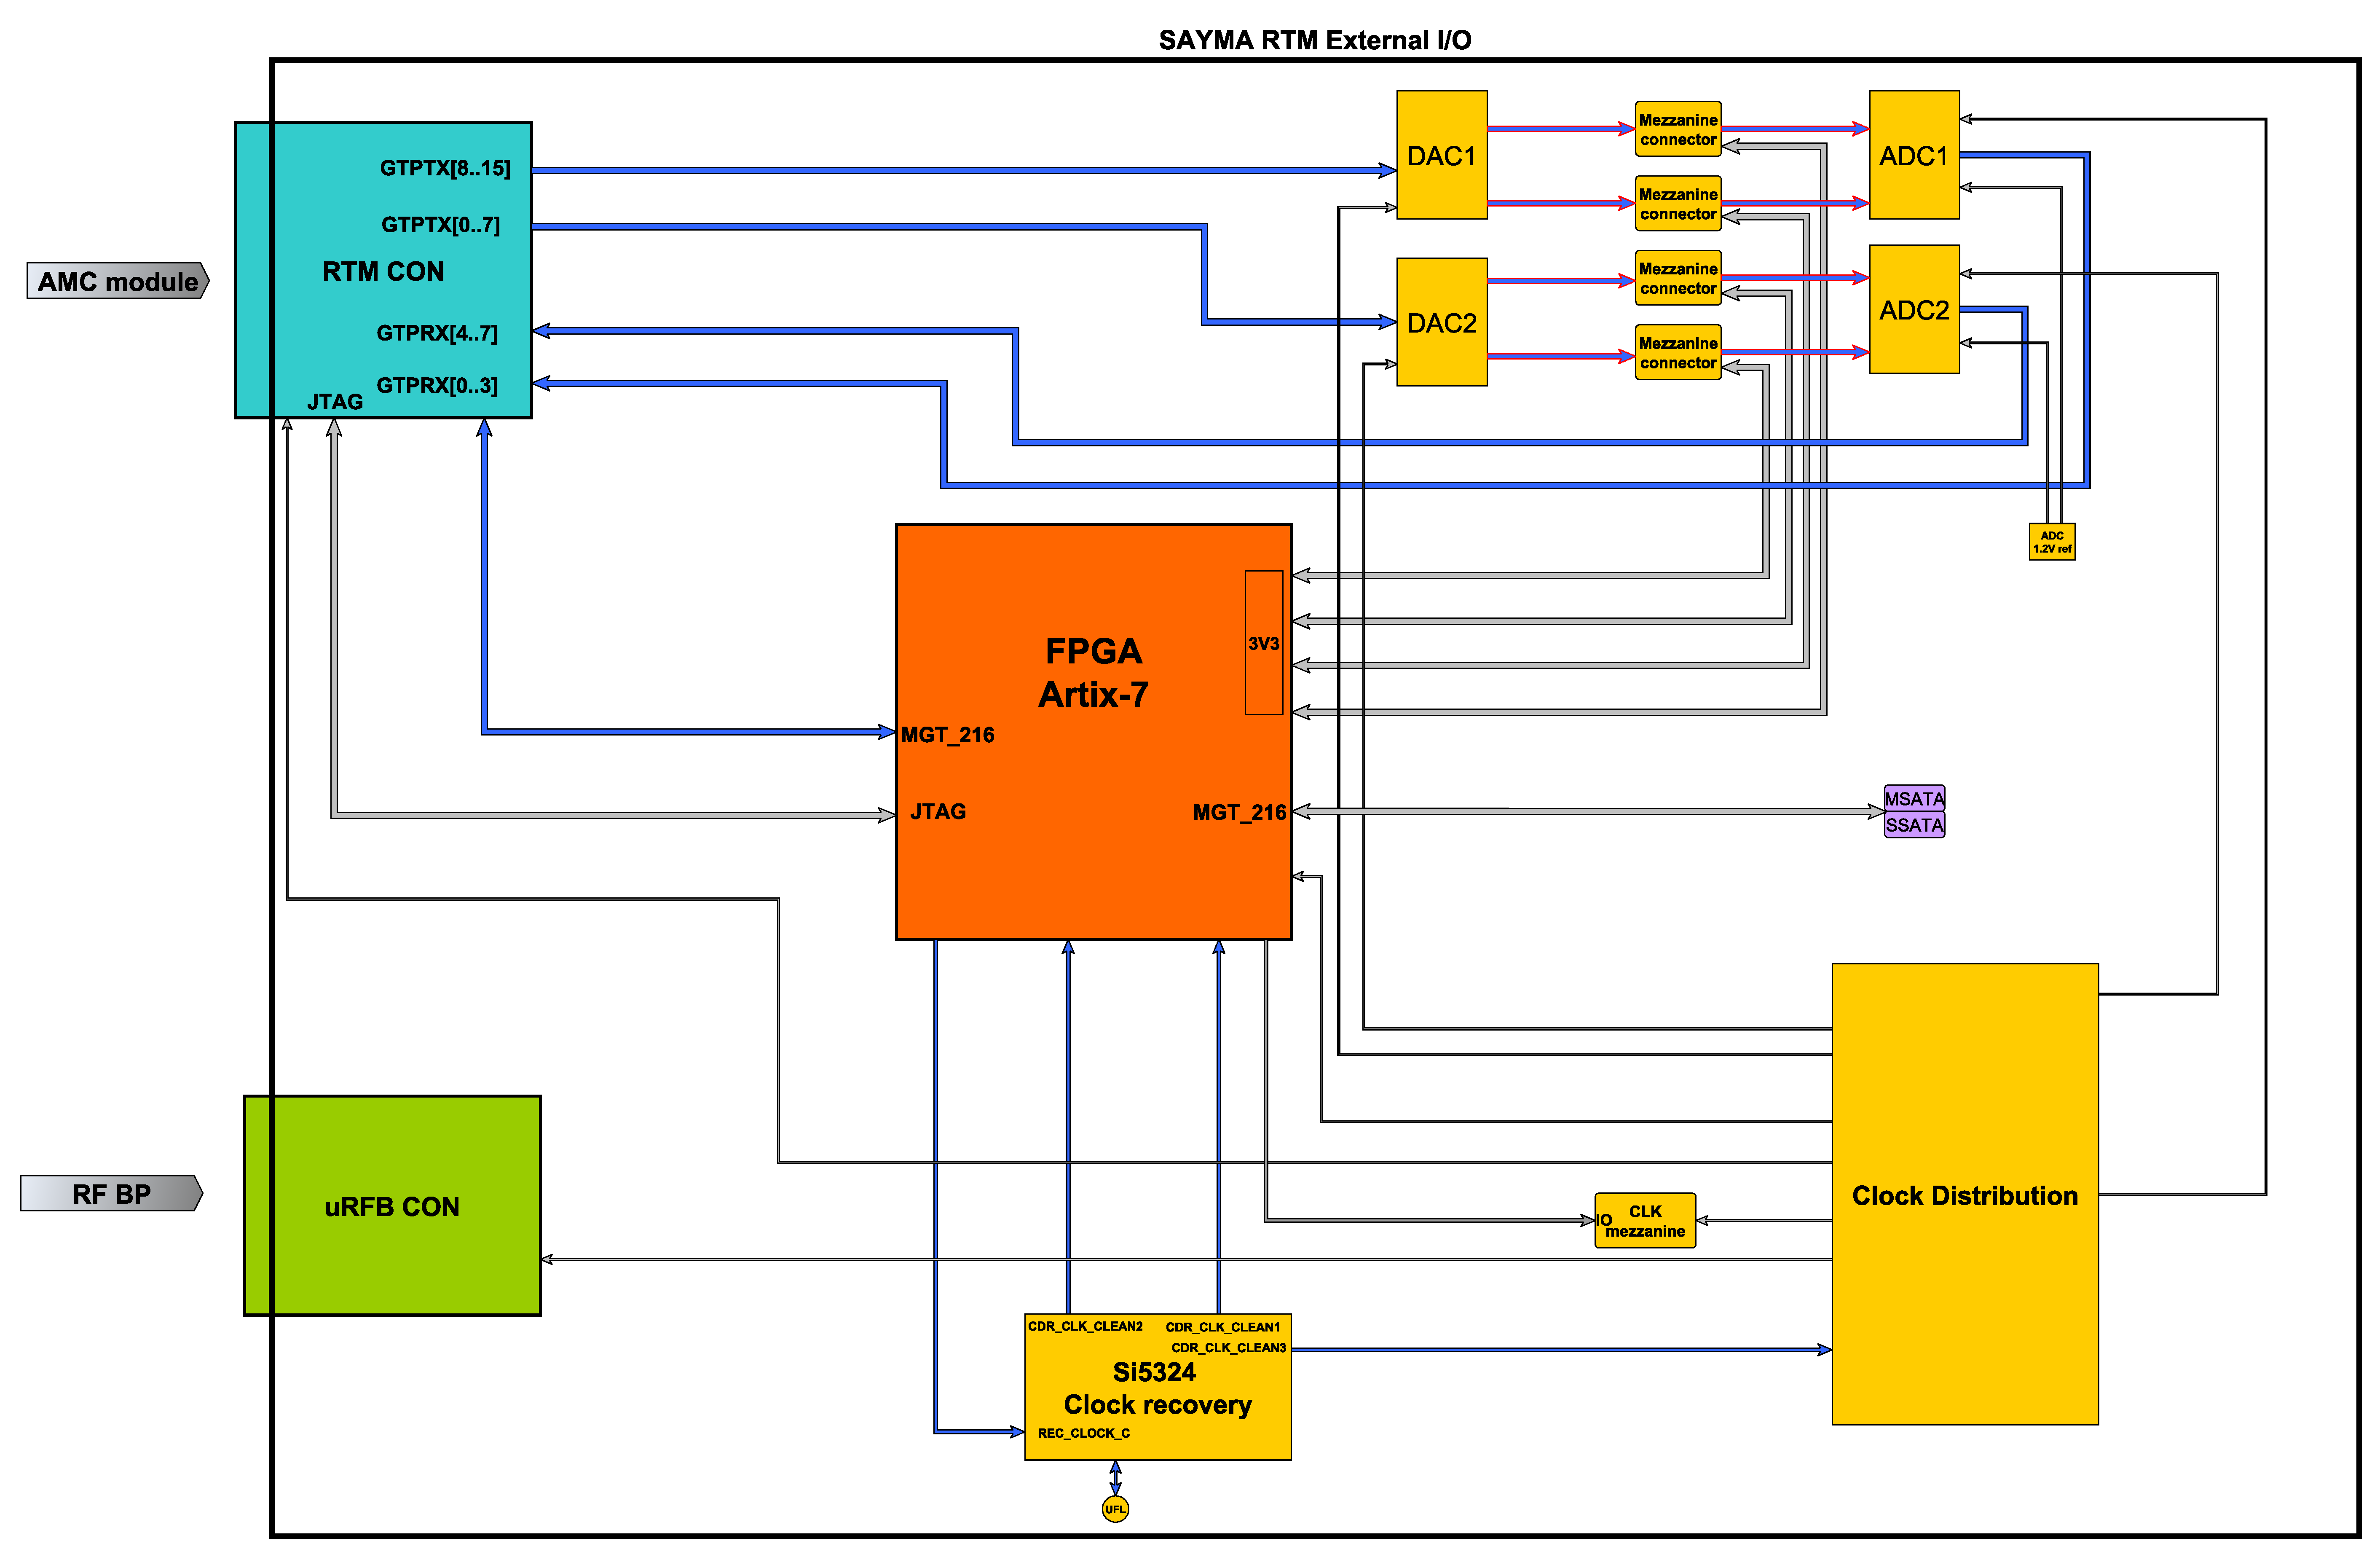
\includegraphics[width=17cm]{img/sch.eps}\\
		\caption{Block Scheme} \label{BlockScheme}
	\end{figure}
\clearpage
The I2C MUX is made from two (TCA9548ARGER)  I2C multiplexers. In Sayma AMC there are two main I2C busses: MMC\_I2C and FPGA\_I2C. Each of them is connected to one multiplexer. Outputs are tied together, so Masters (MMC and FPGA) can acces to any of 7 I2C busses. Addidtionaly MMC has acces to FPGA\_I2C and is connected to IPMB through AMC connector.\\  
	\begin{figure}[htbp!]
		\centering
		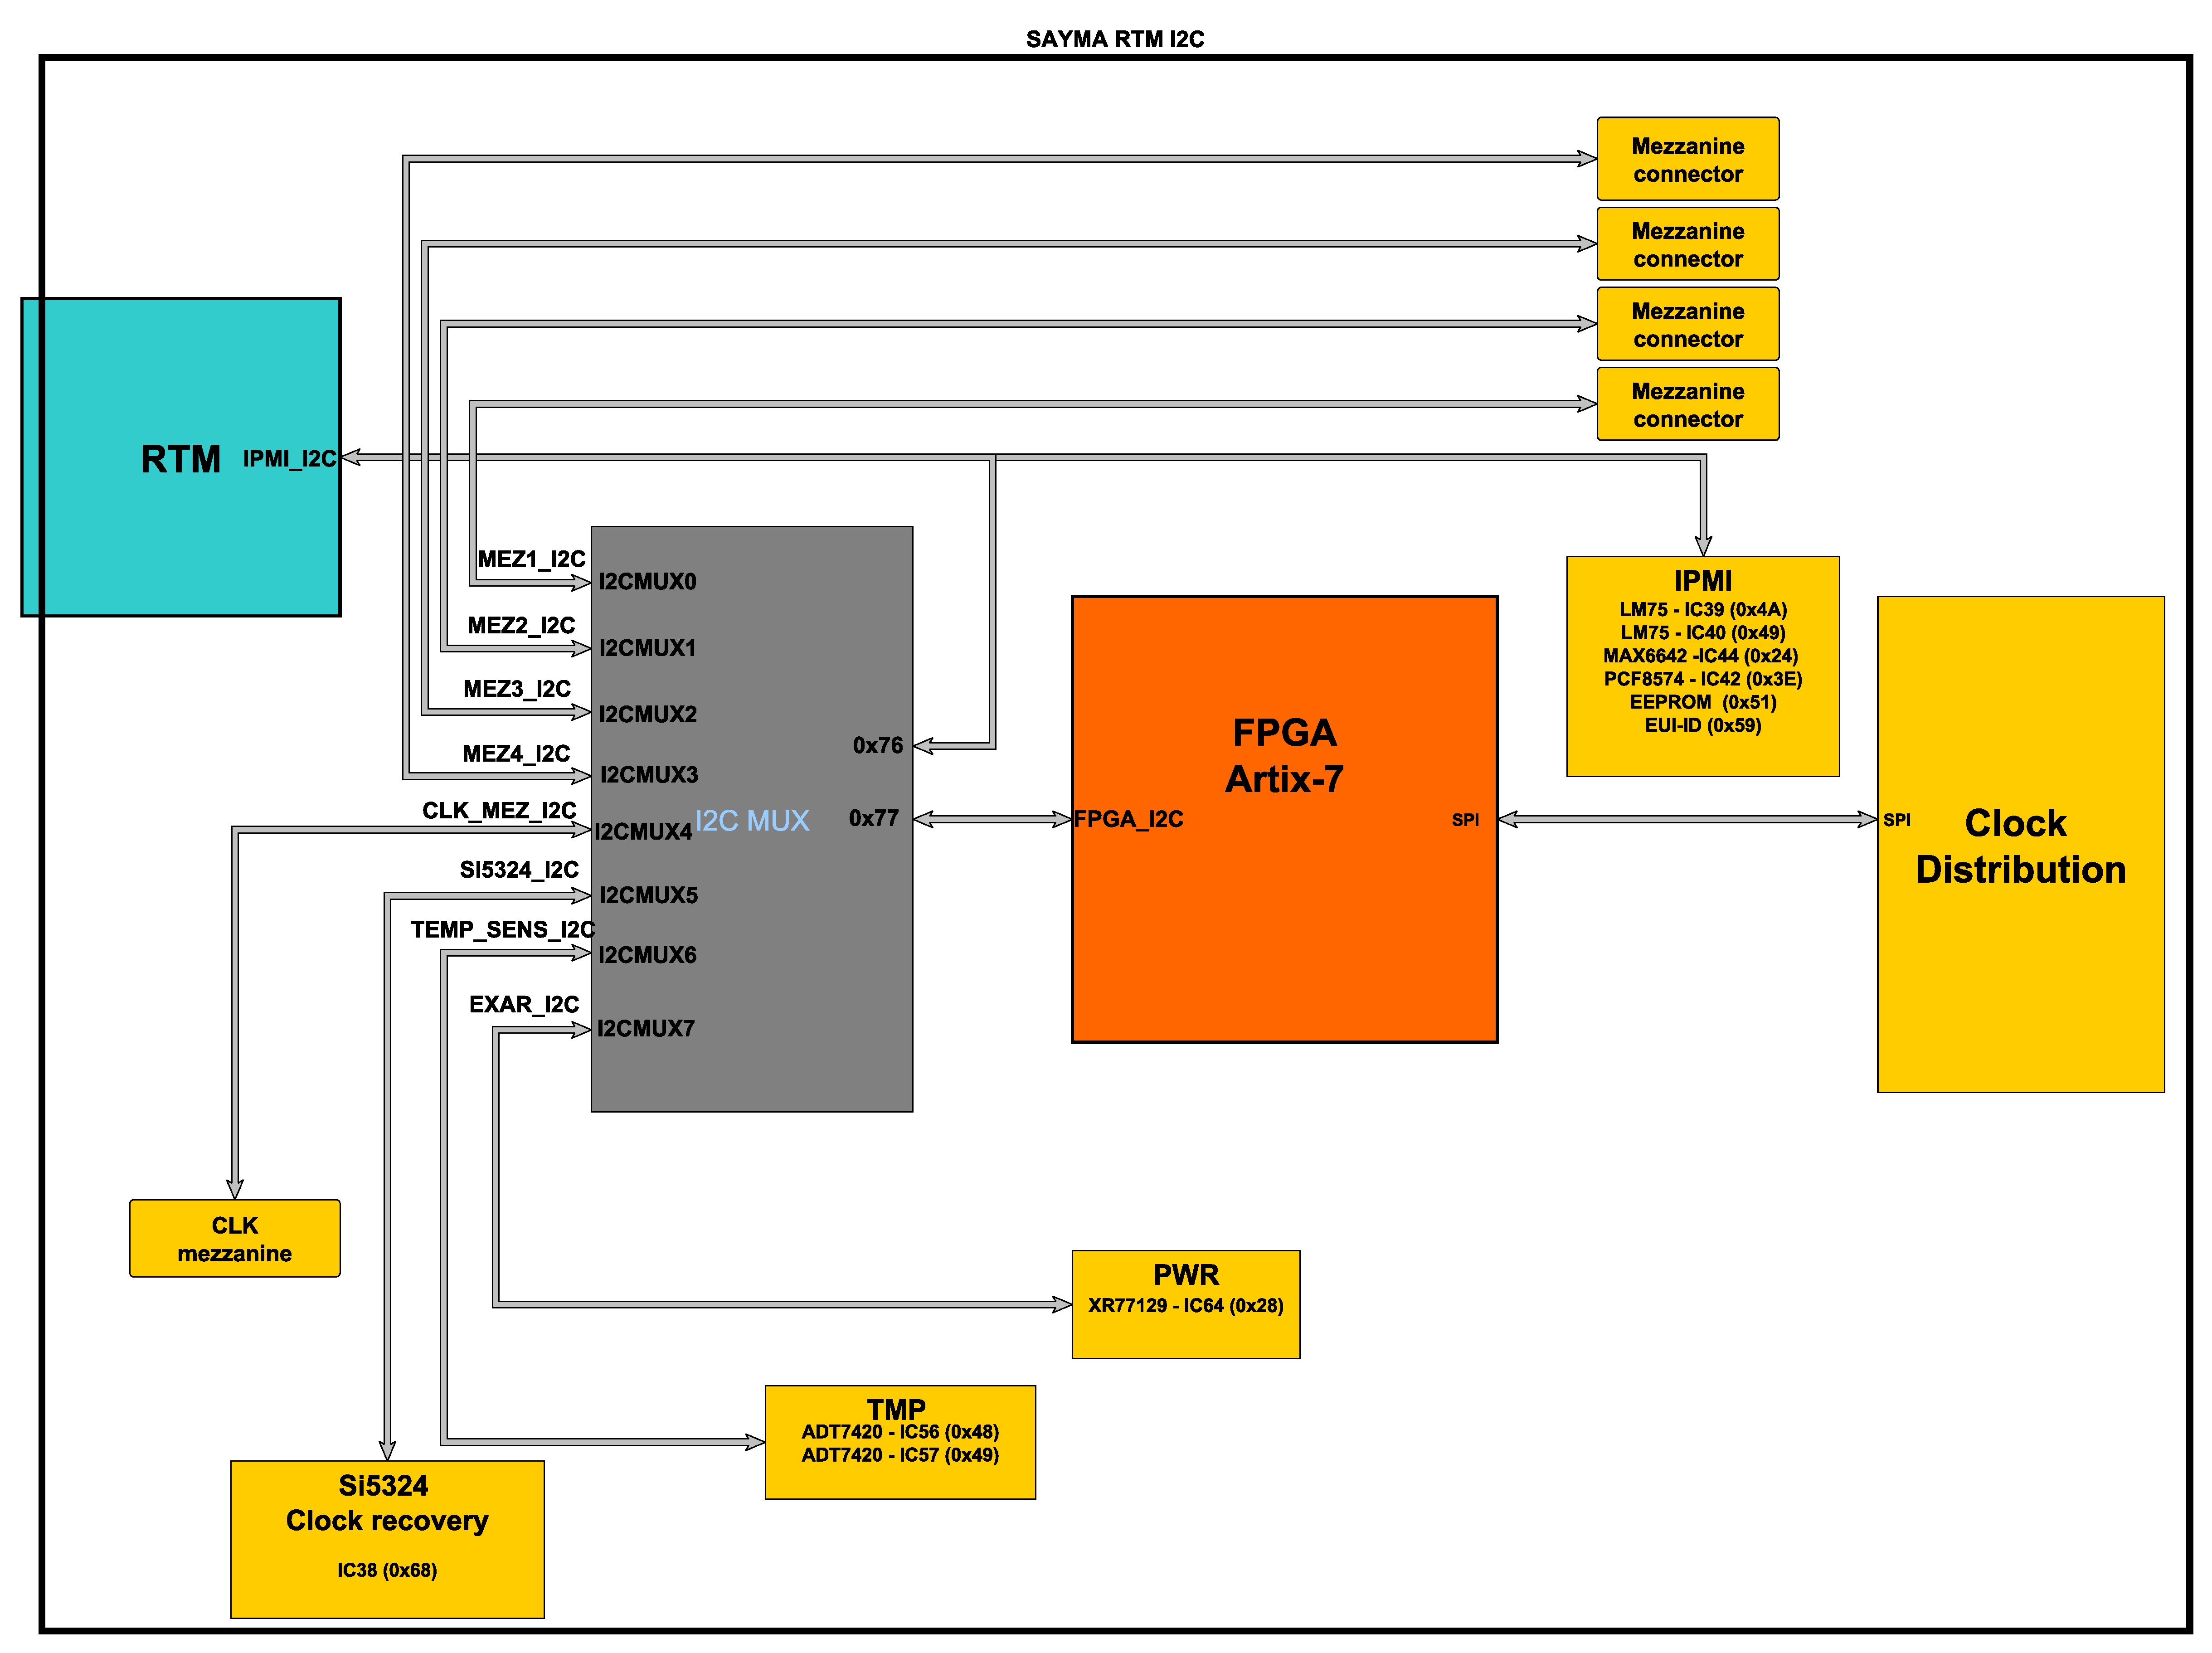
\includegraphics[width=17cm]{img/i2c.eps}\\
		\caption{I2C} \label{I2C}
	\end{figure}

